\documentclass[a4paper]{article}

\usepackage[brazilian]{babel}
\usepackage[utf8x]{inputenc}
\usepackage[T1]{fontenc}

\usepackage{float}

\usepackage{listings}
\usepackage{pythonhighlight}

%% Useful packages
\usepackage{amsmath}
\usepackage{graphicx}
\usepackage[colorinlistoftodos]{todonotes}
\usepackage[colorlinks=true, allcolors=blue]{hyperref}

\usepackage{mathrsfs}
\usepackage{amssymb}



%opening
\title{Relatório do Projeto 2}
\author{Daniel Moreira Cestari - 5746193}

\begin{document}

\maketitle

\section{Introdução}

O objetivo do Projeto 2 é o desenvolvimento de uma triangulação Delaunay 2D.  

A entrada do algoritmo é um conjunto de pontos

A especificação do projeto pede para gerar uma malha dados, uma distância $D$ entre um círculo de raio $R$ e a borda esquerda do domínio retangular, o domínio tem comprimento $L$ e deve ser dividido em $k$ partições. Sendo que, uma dessas partições necessariamente precisa dividir o círculo em dois. O círculo deve estar centrado no domínio em termos da coordenada vertical. Também é pedido para refinar a malha ao redor do círculo e no centro do domínio à direita do círculo.

A maneira de como o círculo é gerado, como as partições e o refinamento são feitos não estão definidos, sendo livre a escolha.


\section{Implementação}

Nesta seção é apresentada a implementação do código, e o porque de determinadas escolhas.

Basicamente o código está dividido em 3 partes:
\begin{itemize}
	\item \textbf{Geração da curva e domínio}: Nesta etapa é gerada a curva e os limites do domínio baseado nos parâmetros passados. Também é possível ler uma curva de um arquivo ou passar uma função que gere outra curva, tornando a implementação mais genérica.
	
	\item \textbf{Particionamento do domínio e determinação dos bordos}: Basicamente o particionamento do domínio tem apenas duas restrições, dividir a curva no meio e realizar um número $k+1$ de partições ($k$ é o parâmetro passado que determina quantos pontos de quebra o eixo $x$ tem).
	Foram implementadas duas maneiras de determinação dos bordos, chamadas de heurística 1 e 2.
	
	\item \textbf{Geração da malha}: Esta é a única etapa que utiliza código já implementado dos exercícios práticos. Após as várias partições serem geradas, cada uma têm sua malha gerada resolvendo a equação de \textit{Laplace} e ao final são unidas em duas malhas que são refinadas na região desejada.
	
\end{itemize}

A seguir, cada etapa será descrita com mais detalhes.


\subsection{Geração da curva e domínio}

A geração da curva, no caso um círculo, é realizada por uma função \textit{circle} que recebe 3 parâmetros. Abaixo é exibido o trecho do código com a função.

%%%%%%%%%%%%%%%%%%%%
% def circle
\inputpython{project1.py}{8}{20}
%%%%%%%%%%%%%%%%%%%%

A convenção adotada na geração da curva é começar do ponto mais a direita em $x$ e seguir o sentido anti-horário.
Uma alternativa à geração do círculo, é a leitura de uma curva em arquivo, como o arquivo \textit{naca012.txt} já utilizado em um exercício prático, ou passar uma função que gere outra curva.

%%%%%%%%%%%%%%%%%%%%
% def generate_curve
\inputpython{project1.py}{25}{75}
%%%%%%%%%%%%%%%%%%%%


Na \textit{docstring} é apresentada uma descrição geral da função e de cada parâmetro.
A função \textit{generate\_curve} retorna um dicionário com os pontos que definem o domínio e a curva.


\subsection{Particionamento do domínio e determinação dos bordos}

A função \textit{partitionate\_domain} chama as funções que realizam o particionamento e determinação dos bordos, \textit{heuristic\_1} e \textit{heuristic\_2}. Para a reutilização do código que resolve a equação de \textit{Laplace} cada partição é salva em arquivo, e essa função que salva cada partição em arquivo.
Abaixo é mostrada a função.

%%%%%%%%%%%%%%%%%%%%
% def partitionate_domain
\inputpython{project1.py}{438}{484}
%%%%%%%%%%%%%%%%%%%%

A diferença entre as duas heurísticas está na divisão feita sobre as partições que contém o círculo.

A primeira heurística (função \textit{heuristic\_1}), na partição do círculo, define o bordo de cima como a parte de cima do domínio mais a reta vertical até chegar ao círculo, e o mesmo princípio para o bordo de baixo, seguindo o sentido da esquerda para a direita. Os bordos da esquerda e direita são definidos pela reta vertical e pela curva, dependendo se a partição está a direita ou a esquerda da curva, e seguindo o sentido de baixo para cima.
As figuras \ref{fig:heuristic1_top1} e \ref{fig:heuristic1_top2} mostram as malhas geradas pela heurística 1 nas partições do círculo. As cores definem os bordos, azul bordo de cima, laranja bordo de baixo, verde bordo da esquerda, e vermelho bordo da direita.

Após a apresentação do trabalho foi incorporado o refinamento dos bordos na heurística 1, e foram removidas as singularidades, quadriláteros com um dos lados de comprimento zero.


 \begin{figure}[h]
 	\centering
 	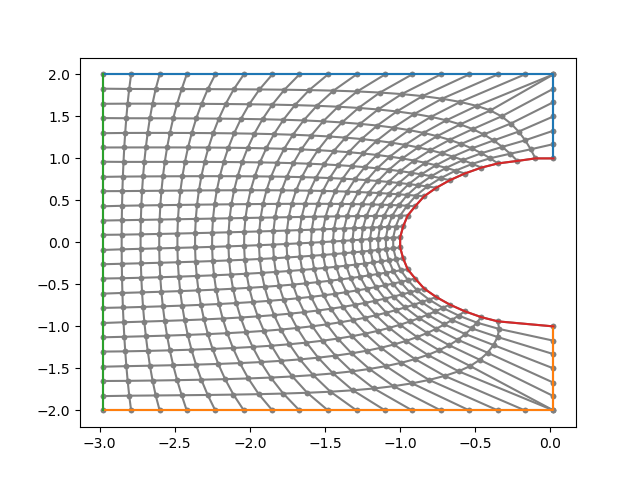
\includegraphics[width=1.0\textwidth]{heuristica_1_50pts_top1.png}
 	\label{fig:heuristic1_top1} 
 	\caption[caption]{Malha gerada pela heurística 1 na primeira metade do círculo}
 \end{figure}


 \begin{figure}[h]
	\centering
	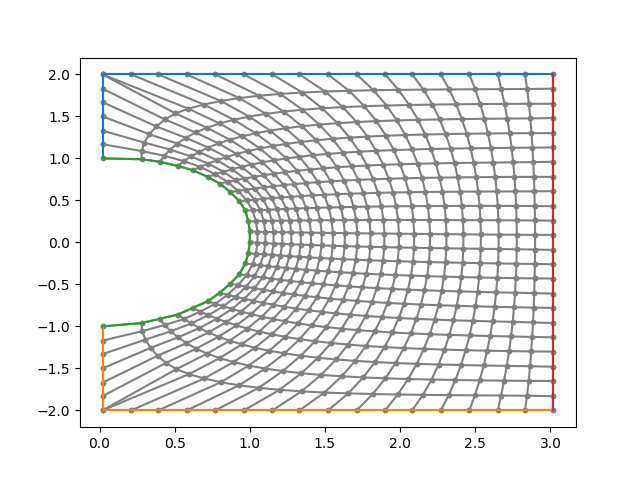
\includegraphics[width=1.0\textwidth]{heuristica_1_50pts_top2.png}
	\label{fig:heuristic1_top2} 
	\caption[caption]{Malha gerada pela heurística 1 na segunda metade do círculo}
\end{figure}


%%%%%%%%%%%%%%%%%%%%
% def heuristic_1
\inputpython{project1.py}{78}{256}
%%%%%%%%%%%%%%%%%%%%





A heurística 2 difere da 1, na sua definição dos bordos sobre a partição da curva. Neste caso, a divisão é feita seguindo o lado, se lado em questão está a esquerda então é o bordo esquerdo, se está a direita é o bordo direito, se está acima é o de cima e se está abaixo o de baixo. Esta heurística não apresenta refinamento nos bordos.
As figuras \ref{fig:heuristic2_top1} e \ref{fig:heuristic2_top2} mostram malhas geradas utilizando a heurística 2, as cores têm o mesmo significado que o relatado na heurística 1.


\begin{figure}[h]
	\centering
	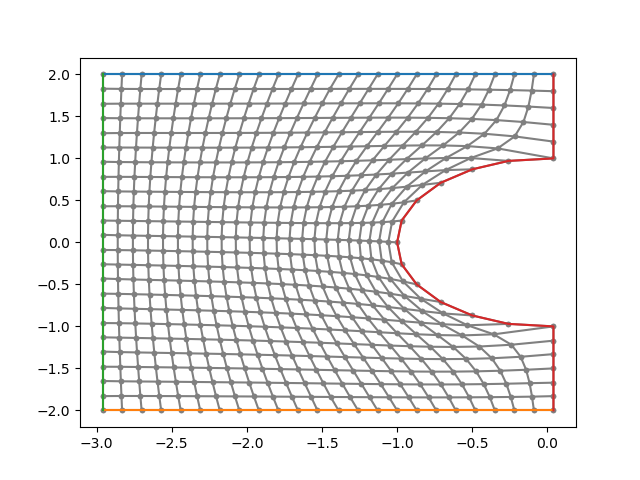
\includegraphics[width=1.0\textwidth]{heuristica_2_25pts_top1.png}
	\label{fig:heuristic2_top1} 
	\caption[caption]{Malha gerada pela heurística 2 na primeira metade do círculo}
\end{figure}


\begin{figure}[h]
	\centering
	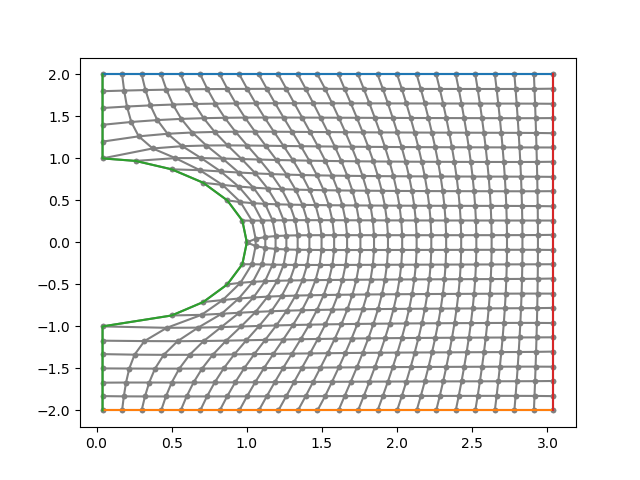
\includegraphics[width=1.0\textwidth]{heuristica_2_25pts_top2.png}
	\label{fig:heuristic2_top2} 
	\caption[caption]{Malha gerada pela heurística 2 na segunda metade do círculo}
\end{figure}


%%%%%%%%%%%%%%%%%%%%
% def heuristic_2
\inputpython{project1.py}{260}{433}
%%%%%%%%%%%%%%%%%%%%


\subsection{Geração da malha}

A função que gera a malha chama as funções que criam o domínio e o particionam, e depois resolve a equação de \textit{Laplace} em cada partição individualmente. Após a malha de cada partição ser gerada, elas são unidas em duas malhas e então o refinamento é realizado resolvendo a equação de \textit{Poisson} nas duas malhas finais. Mesmo que um refinamento utilizando as funções de controle não seja realizado, como a equação de \textit{Laplace} é utilizada novamente com as malhas unidas, é feita uma suavização nos pontos de união das malhas.

Essa é a principal função que chama todas as outras necessárias, e por isso é cheia de parâmetros. Todos descritos na \textit{docstring}, basicamente juntou todos os parâmetros das funções anteriores mais os parâmetros relativos ao refinamento da malha.

Abaixo é apresentada a função \textit{generate\_grid}.

%%%%%%%%%%%%%%%%%%%%
% def generate_grid
\inputpython{project1.py}{489}{729}
%%%%%%%%%%%%%%%%%%%%

O arquivo \textit{VTK} final é o resultado da união das duas malhas finais refinadas. Foi preciso modificar o código original que gerava o \textit{VTK} para receber uma lista de malhas e quando salvar em disco, produzir apenas um arquivo. Foi tomado o cuidado para vértices posicionados na mesma posição não aparecerem repetidos, ou seja, as malhas são realmente unidas.


\section{Resultados}


Nesta seção serão apresentados os resultados obtidos com a implementação descrita anteriormente. Primeiro serão mostradas as malhas para a heurística 1 variando o número de pontos na malha, em seguida será feito o mesmo para a heurística 2.
A configuração do domínio e da curva será a mesma para ambas as heurísticas.

Após a apresentação do trabalho foram apontados algumas correções, agora incorporadas, mas devido às modificações o exemplo utilizando o aerofólio ficou ruim e foi removido deste relatório.

Todos os arquivos VTK gerados foram anexados.

\subsection{Heurística 1}

Código para gerar uma malha com 52 pontos nos bordos esquerdo e direito. Curva gerada com 52 pontos, centrada na origem, domínio com comprimento 10, altura 8, e comprimento 3 à direita da curva. O domínio é divido em 4 partes, e o refinamento é deixado apenas nos bordos e a equação de \textit{Laplace} propaga esse refinamento para o interior do domínio.


\begin{verbatim}
import imp
import numpy as np
from matplotlib import pyplot as plt
import project1 as pjt

imp.reload(pjt);  
grid = pjt.generate_grid(resolution=52, left_border=3, domain_length=10, 
domain_height=4, curve_params={"radius":1}, equation=pjt.circle, 
filename_curve="", heuristic=pjt.heuristic_1, k=3, filename_borders="circle_h1_50pts", plot=True)
\end{verbatim}

Abaixo o código agora utilizando 100 pontos.
\begin{verbatim}
import imp
import numpy as np
from matplotlib import pyplot as plt
import project1 as pjt

imp.reload(pjt);  
grid = pjt.generate_grid(resolution=100, left_border=3, domain_length=10, 
domain_height=4, curve_params={"radius":1}, equation=pjt.circle, 
filename_curve="", heuristic=pjt.heuristic_1, k=3, filename_borders="circle_h1_100pts", plot=True)
\end{verbatim}


%\begin{figure}[H]
%	\centering
%	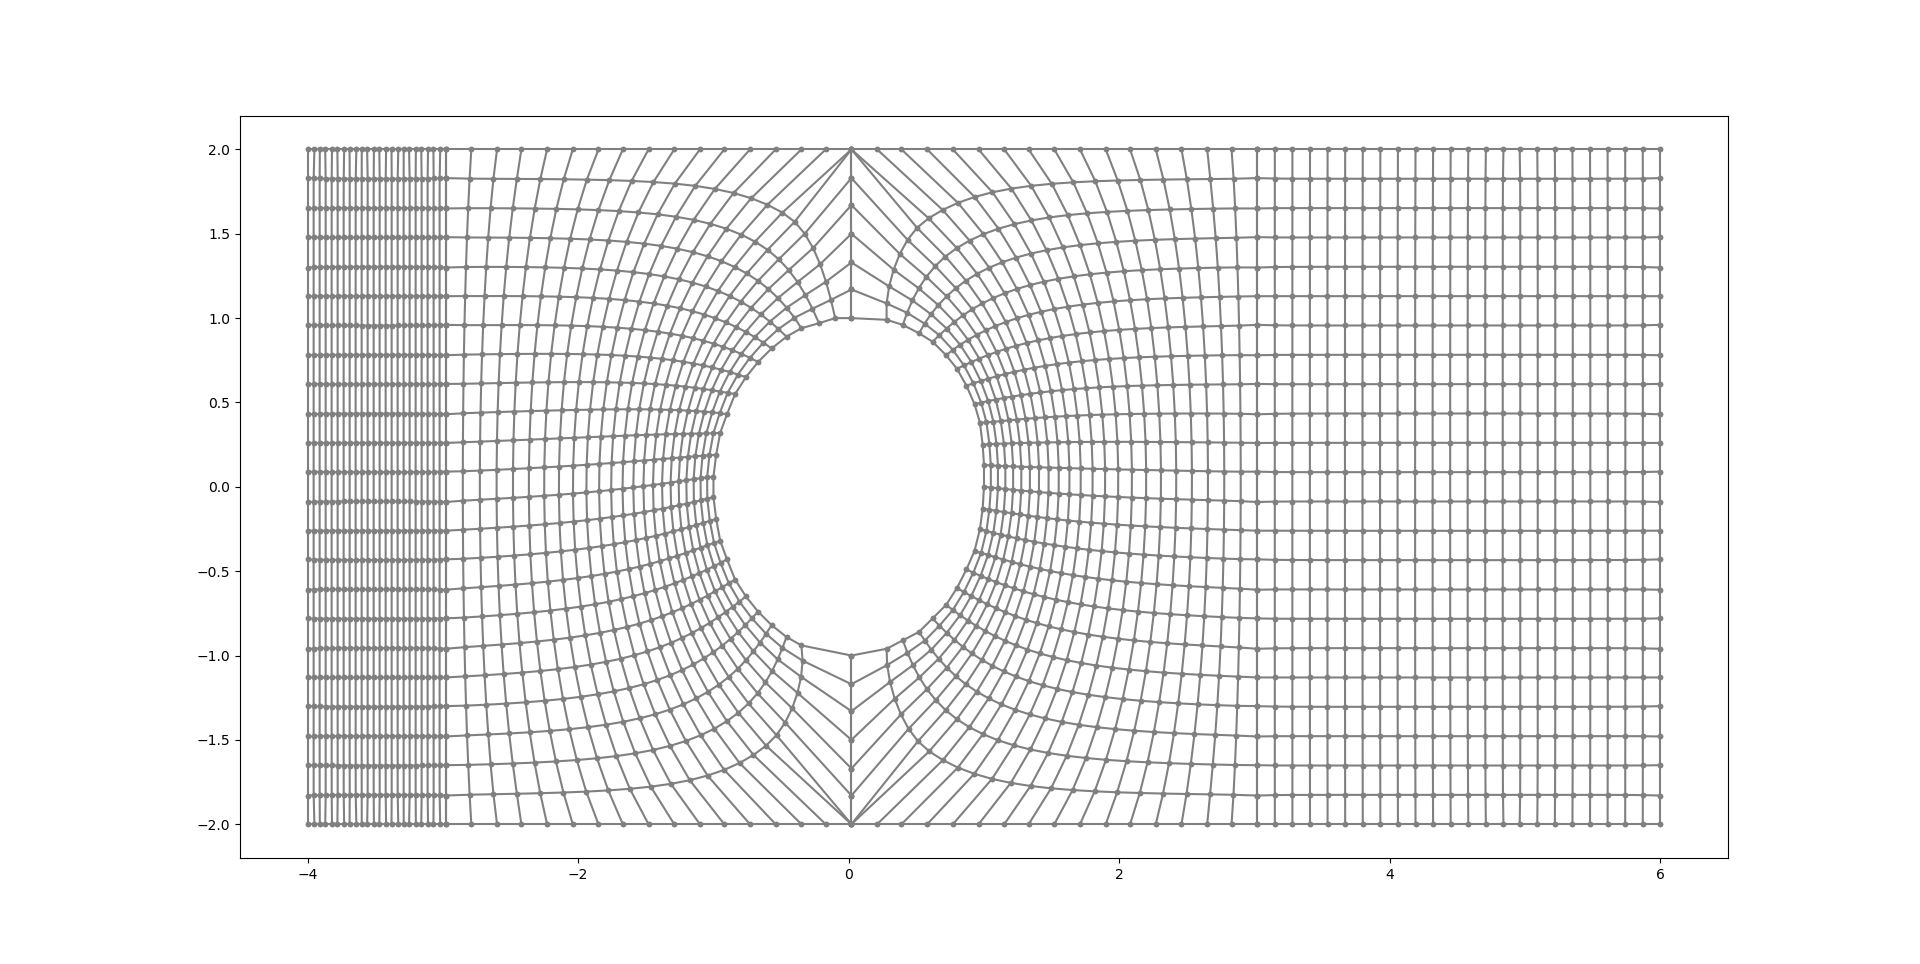
\includegraphics[width=1.0\textwidth]{heuristica_1_50pts.png}
%	\label{fig:heuristic1_50pts} 
%	\caption[caption]{Malha gerada pela heurística 1 com 50 pontos.}
%\end{figure}
%
%\begin{figure}[H]
%	\centering
%	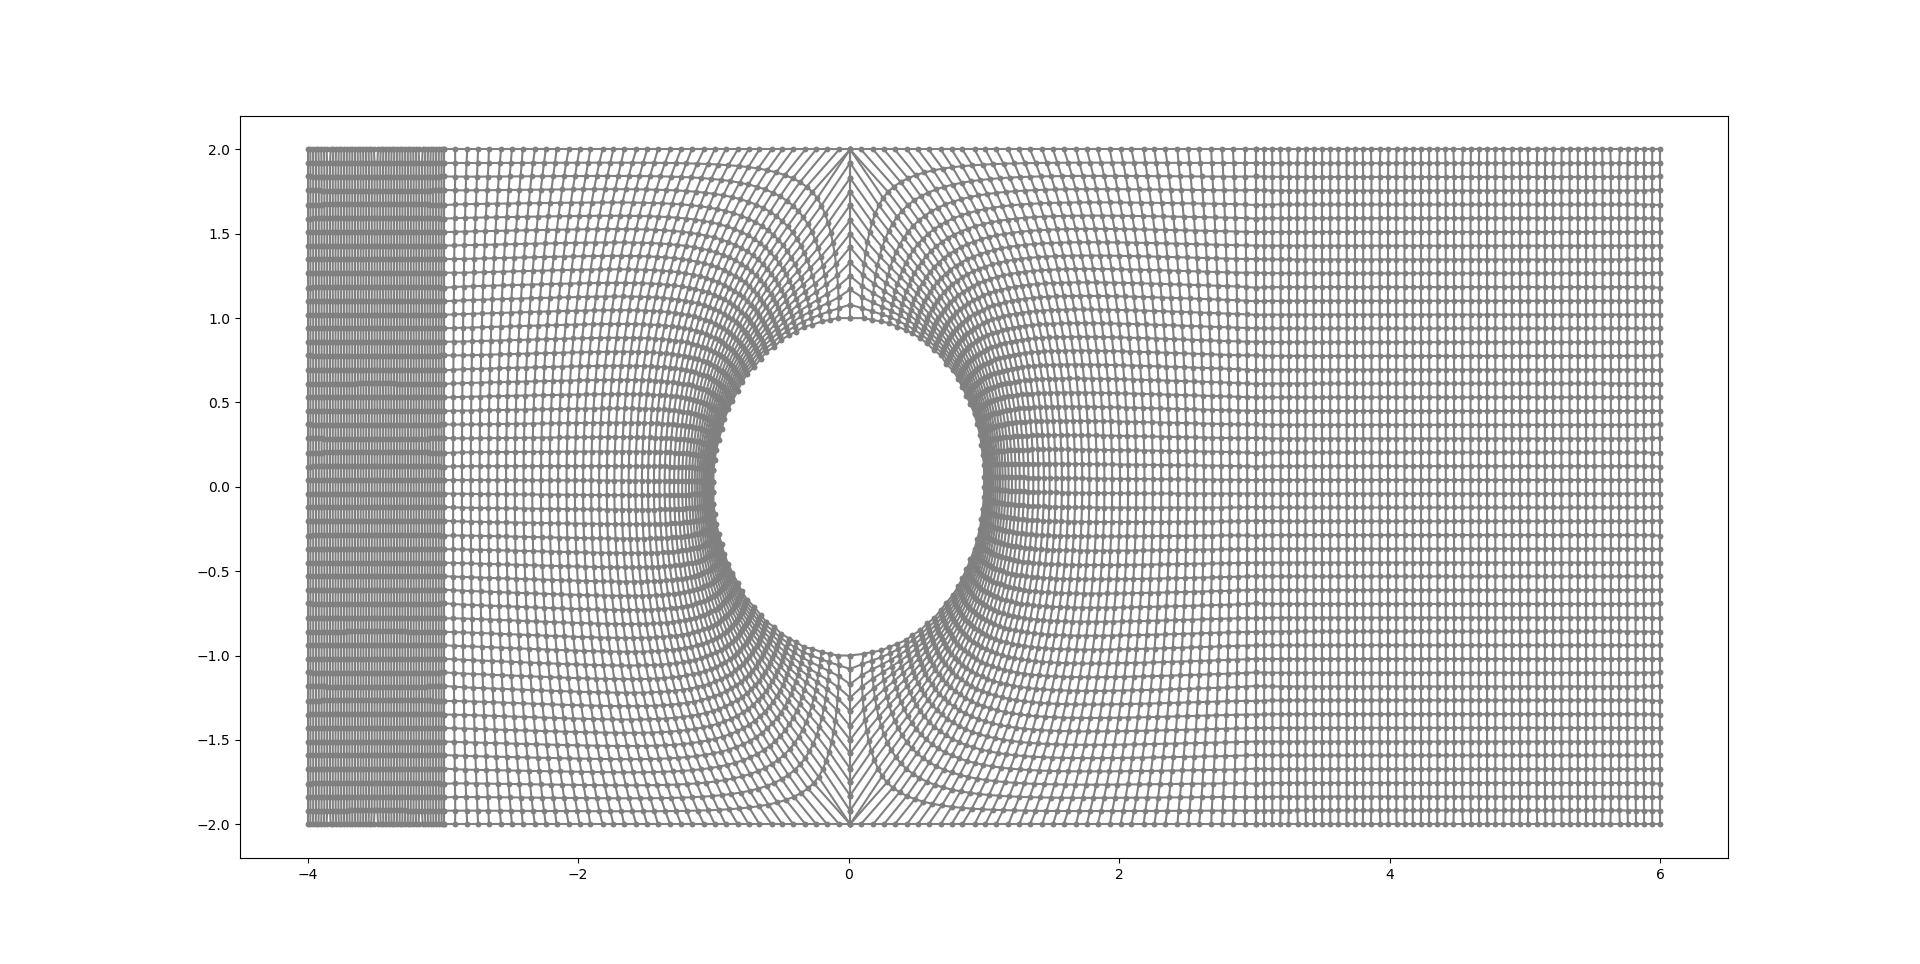
\includegraphics[width=1.0\textwidth]{heuristica_1_100pts.png}
%	\label{fig:heuristic1_100pts} 
%	\caption[caption]{Malha gerada pela heurística 1 com 100 pontos.}
%\end{figure}



\begin{figure}[H]
	\centering
	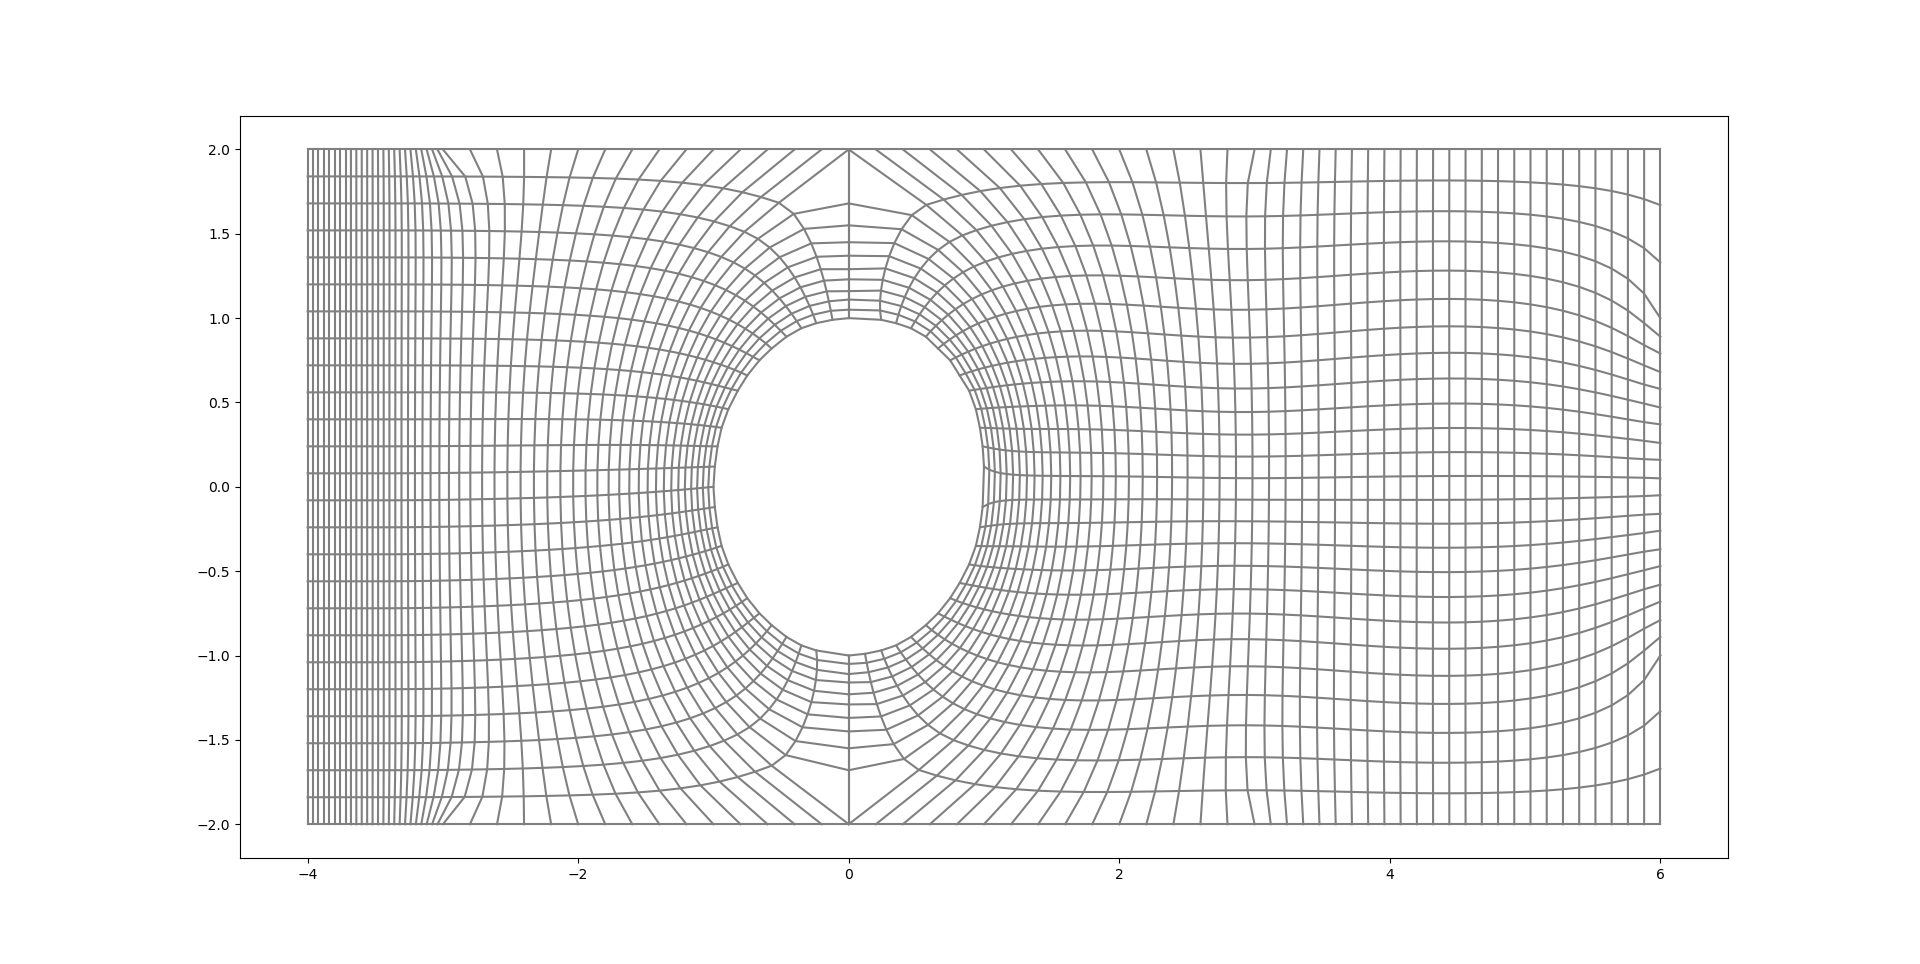
\includegraphics[width=1.0\textwidth]{heuristica_1_52pts_refined.png}
	\label{fig:heuristic1_50pts_refined} 
	\caption[caption]{Malha gerada pela heurística 1 com 52 pontos com refinamento dos bordos.}
\end{figure}

\begin{figure}[H]
	\centering
	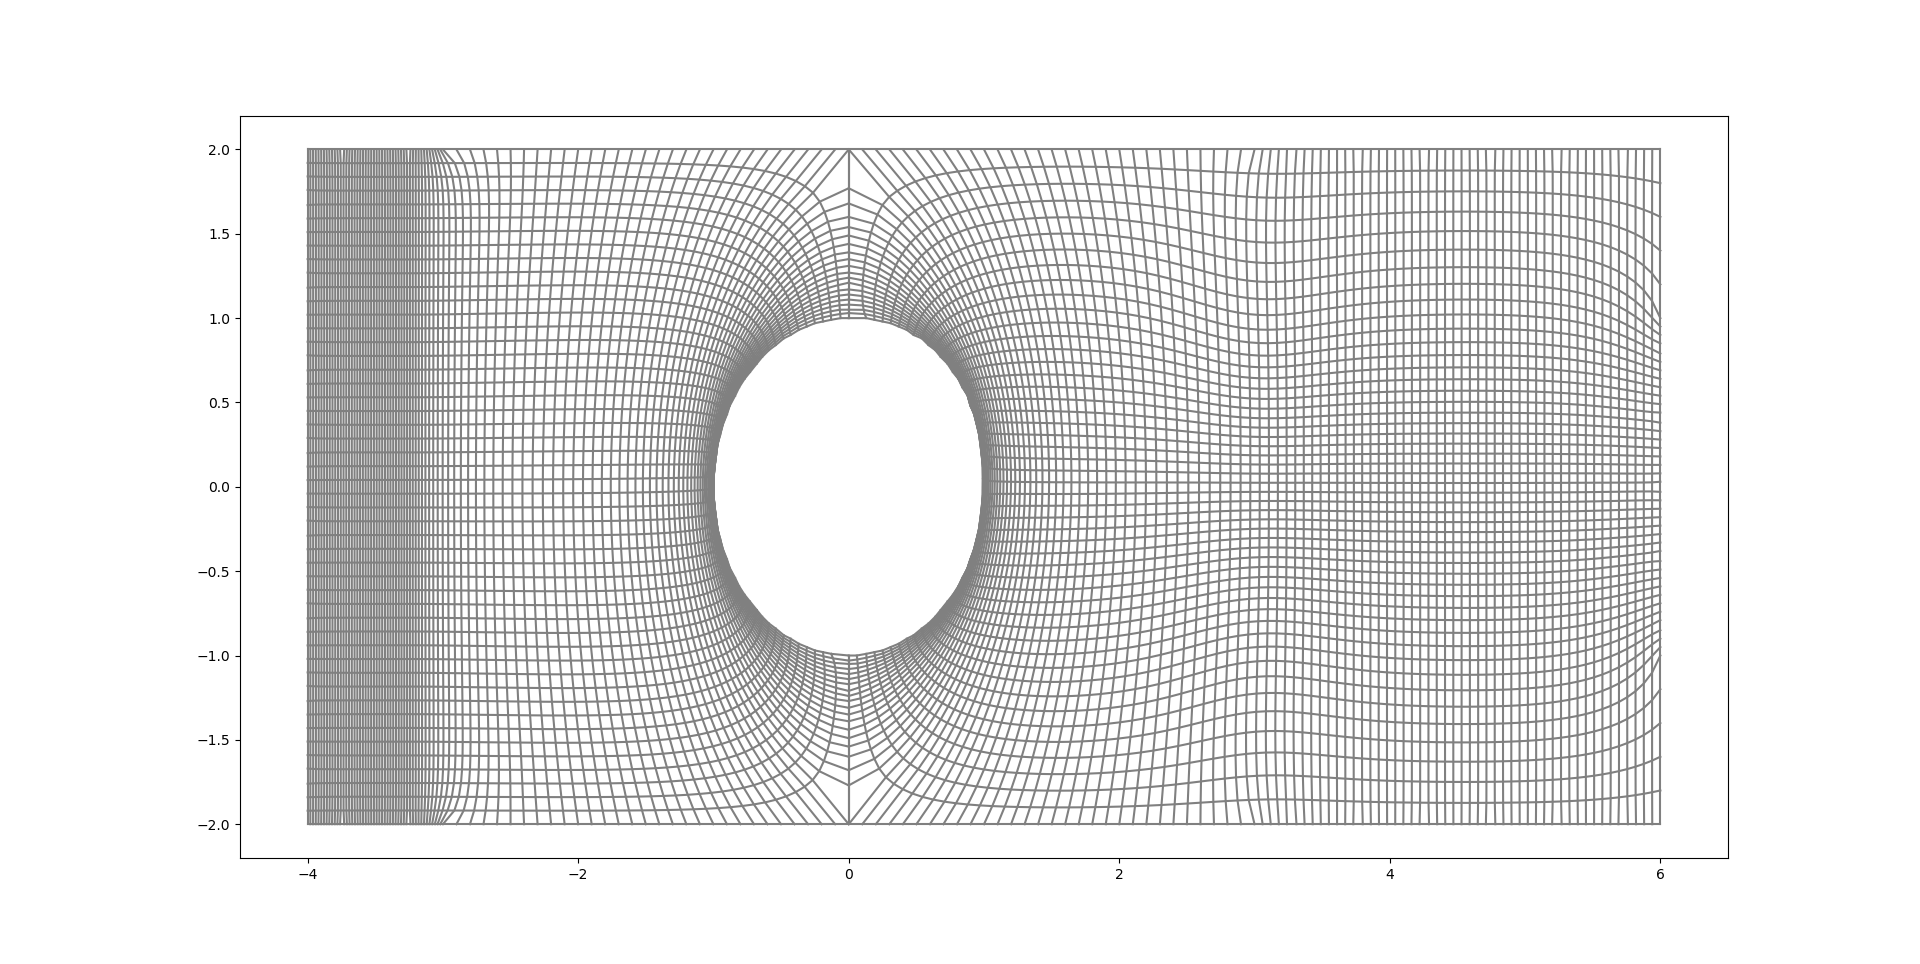
\includegraphics[width=1.0\textwidth]{heuristica_1_100pts_refined.png}
	\label{fig:heuristic1_100pts_refined} 
	\caption[caption]{Malha gerada pela heurística 1 com 100 pontos com refinamento.}
\end{figure}






\subsection{Heurística 2}



Código para gerar uma malha com 25 pontos nos bordos esquerdo e direito. Curva gerada com 25 pontos, centrada na origem, domínio com comprimento 10, altura 8, e comprimento 3 à direita da curva. O domínio é divido em 4 partes, e o refinamento é feito ao redor da curva e após a curva no centro do domínio em relação à \textit{y}, ou $\eta$.

\begin{verbatim}
import imp
import numpy as np
from matplotlib import pyplot as plt
import project1 as pjt

imp.reload(pjt);  
grid = pjt.generate_grid(resolution=25, left_border=3, domain_length=10, 
domain_height=4, curve_params={"radius":1}, equation=pjt.circle, 
filename_curve="", heuristic=pjt.heuristic_2, k=3, filename_borders="circle_h2_25pts", 
xis_rf0=[1], xis_rf1=[0], etas_rf1=[0.45], a_xis0=[2.5], 
a_xis1=[2.5], c_xis0=[5], c_xis1=[5], a_etas1=[0.5], c_etas1=[1], plot=True)
\end{verbatim}

Abaixo o código agora utilizando 50 pontos.
\begin{verbatim}
import imp
import numpy as np
from matplotlib import pyplot as plt
import project1 as pjt

imp.reload(pjt);  
grid = pjt.generate_grid(resolution=50, left_border=3, domain_length=10, 
domain_height=4, curve_params={"radius":1}, equation=pjt.circle, 
filename_curve="", heuristic=pjt.heuristic_2, k=3, filename_borders="circle_h2_50pts", 
xis_rf0=[1], xis_rf1=[0], etas_rf1=[0.45], a_xis0=[5], 
a_xis1=[5], c_xis0=[5], c_xis1=[5], a_etas1=[1], c_etas1=[0.1], plot=True)
\end{verbatim}


%\begin{figure}[H]
%	\centering
%	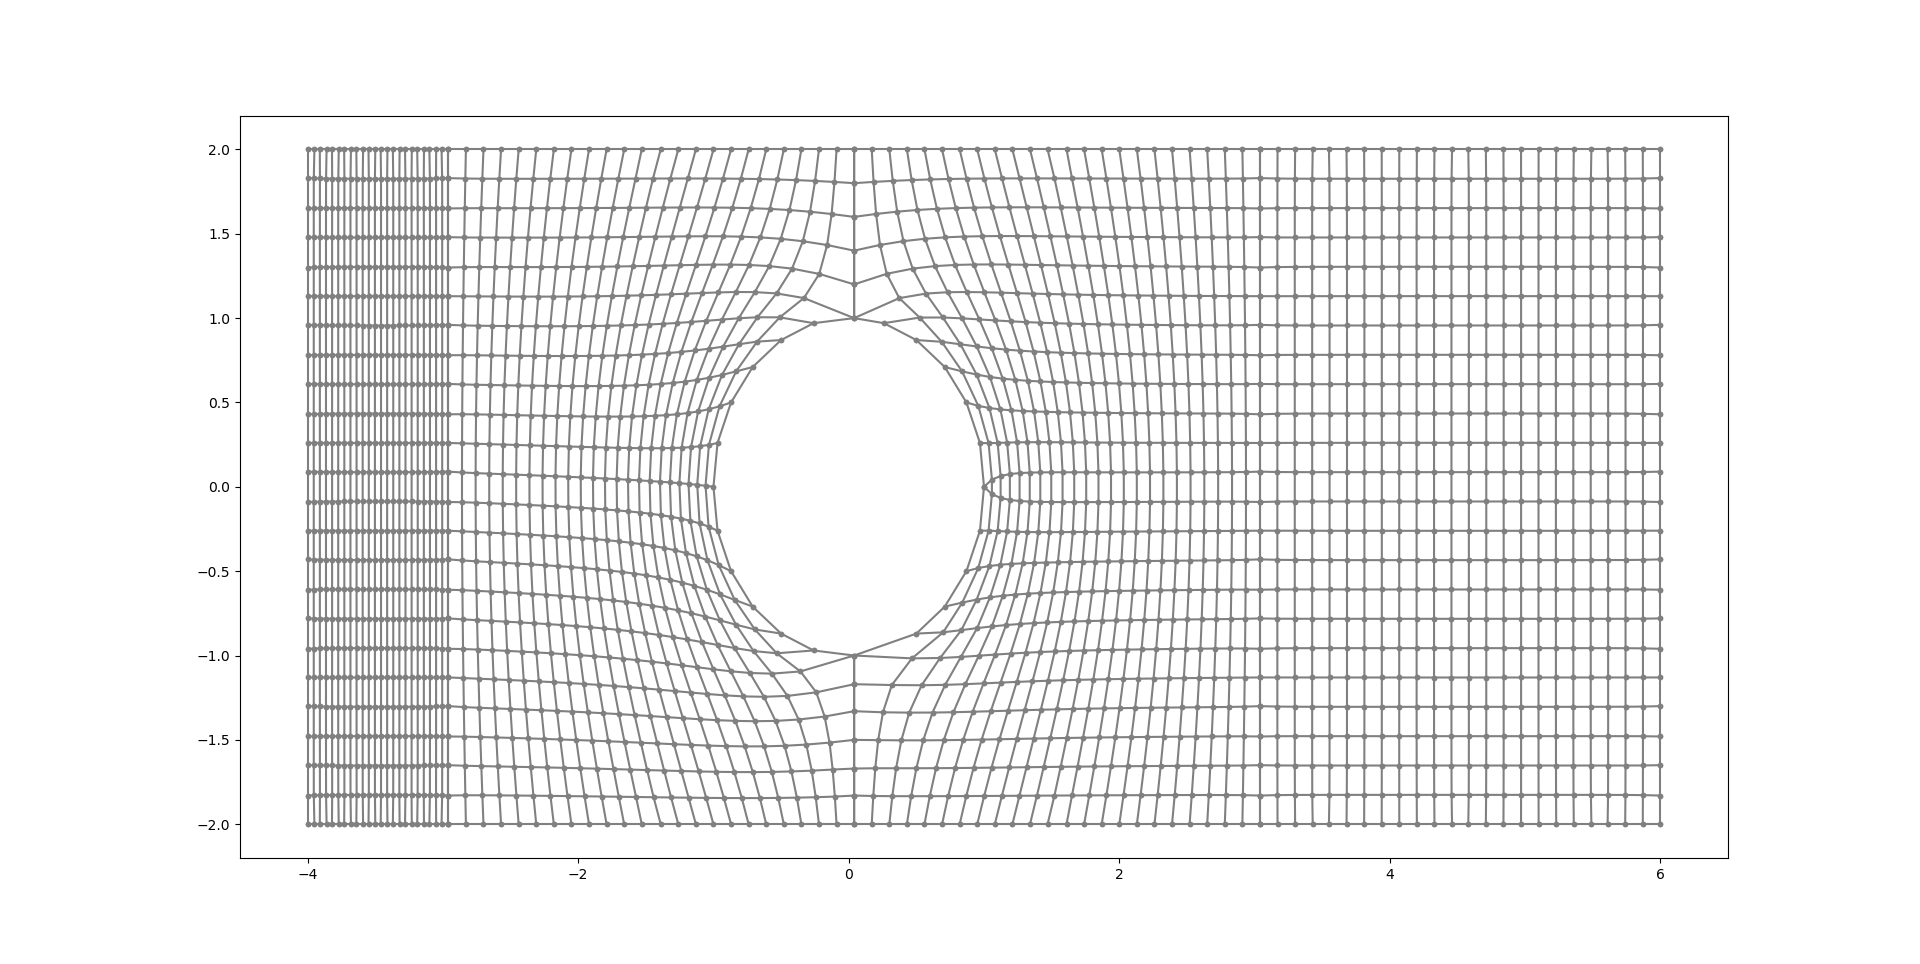
\includegraphics[width=1.0\textwidth]{heuristica_2_25pts.png}
%	\label{fig:heuristic2_50pts} 
%	\caption[caption]{Malha gerada pela heurística 2 com 25 pontos sem refinamento.}
%\end{figure}
%
%\begin{figure}[H]
%	\centering
%	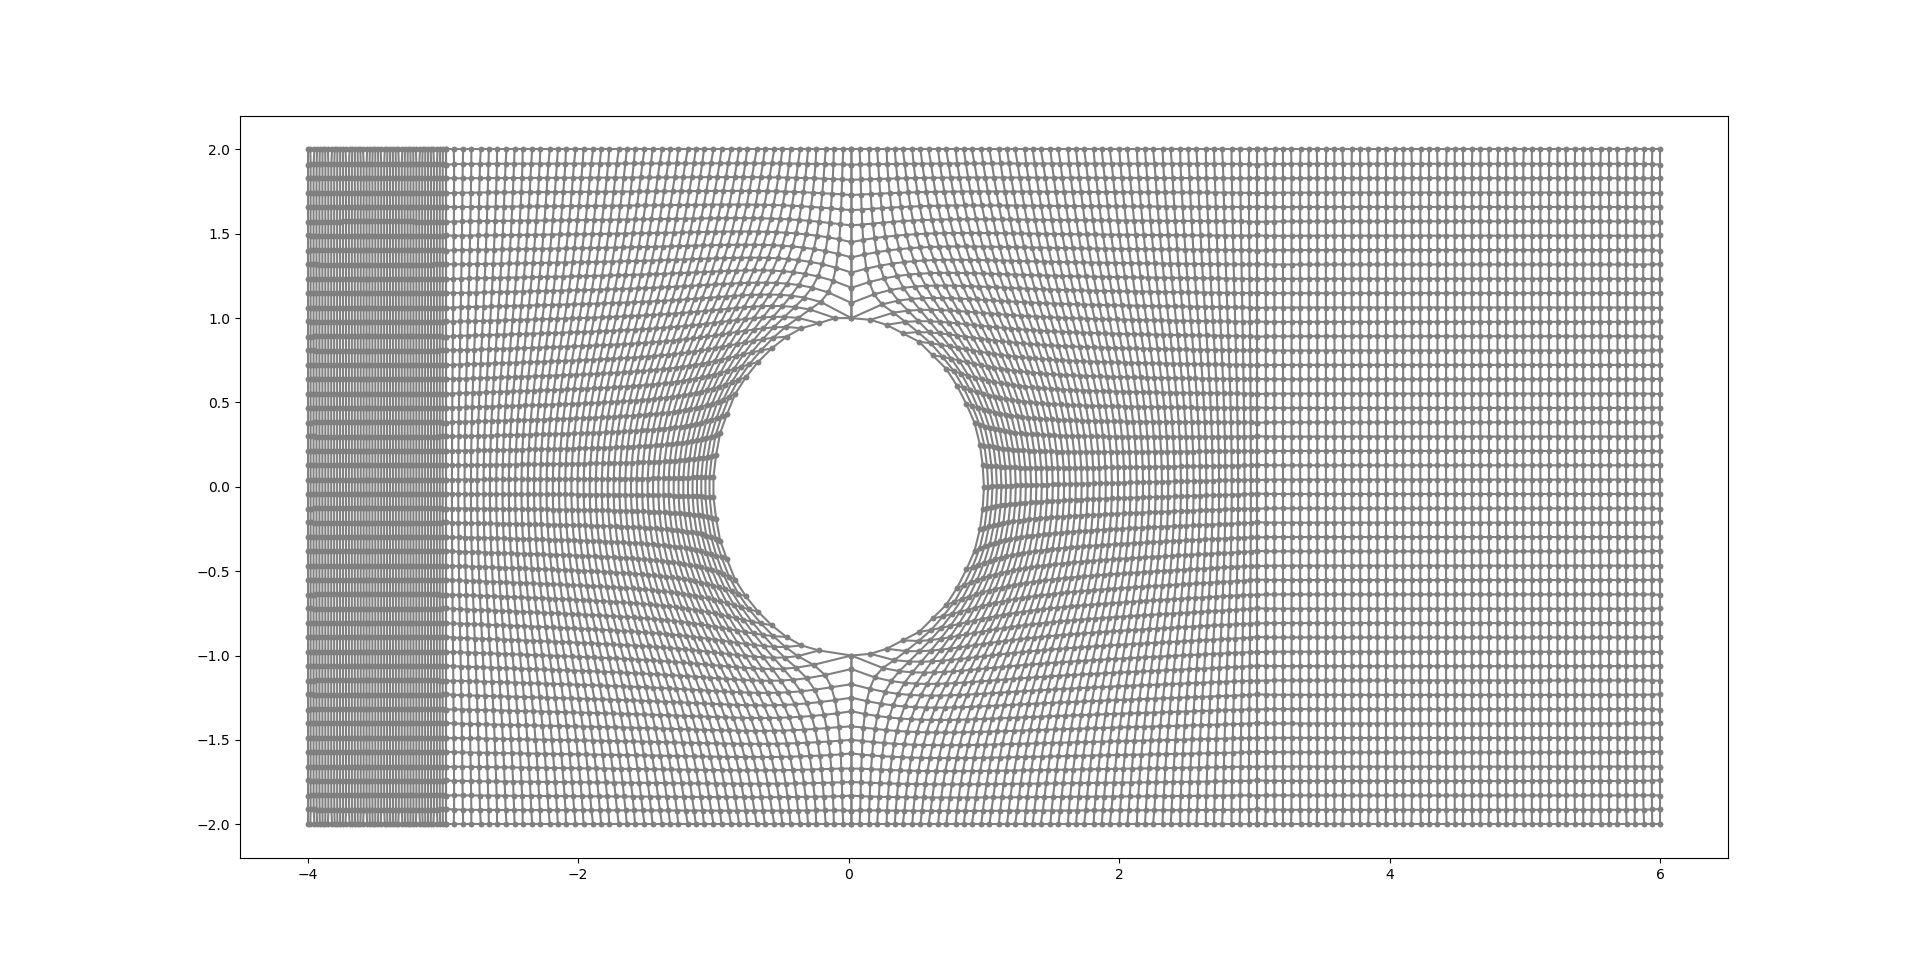
\includegraphics[width=1.0\textwidth]{heuristica_2_50pts.png}
%	\label{fig:heuristic2_100pts} 
%	\caption[caption]{Malha gerada pela heurística 2 com 50 pontos sem refinamento.}
%\end{figure}



\begin{figure}[H]
	\centering
	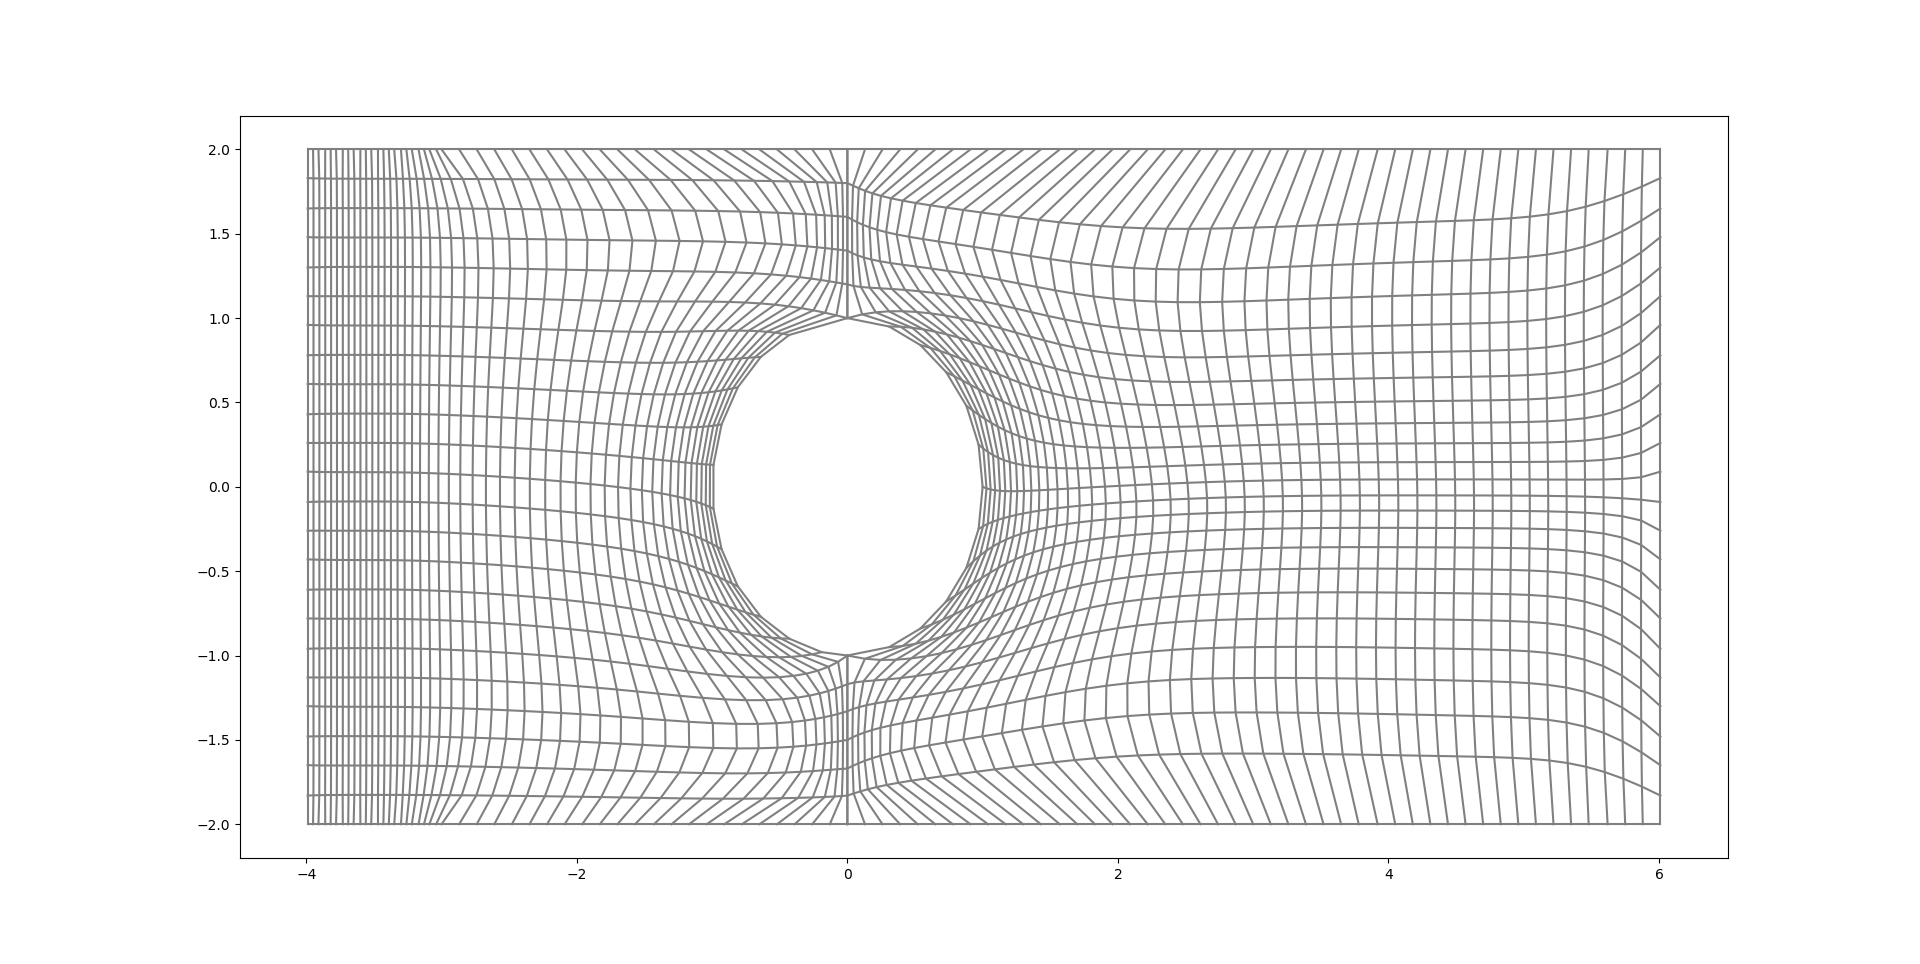
\includegraphics[width=1.0\textwidth]{heuristica_2_25pts_refined.png}
	\label{fig:heuristic2_50pts_refined} 
	\caption[caption]{Malha gerada pela heurística 2 com 25 pontos com refinamento.}
\end{figure}

\begin{figure}[H]
	\centering
	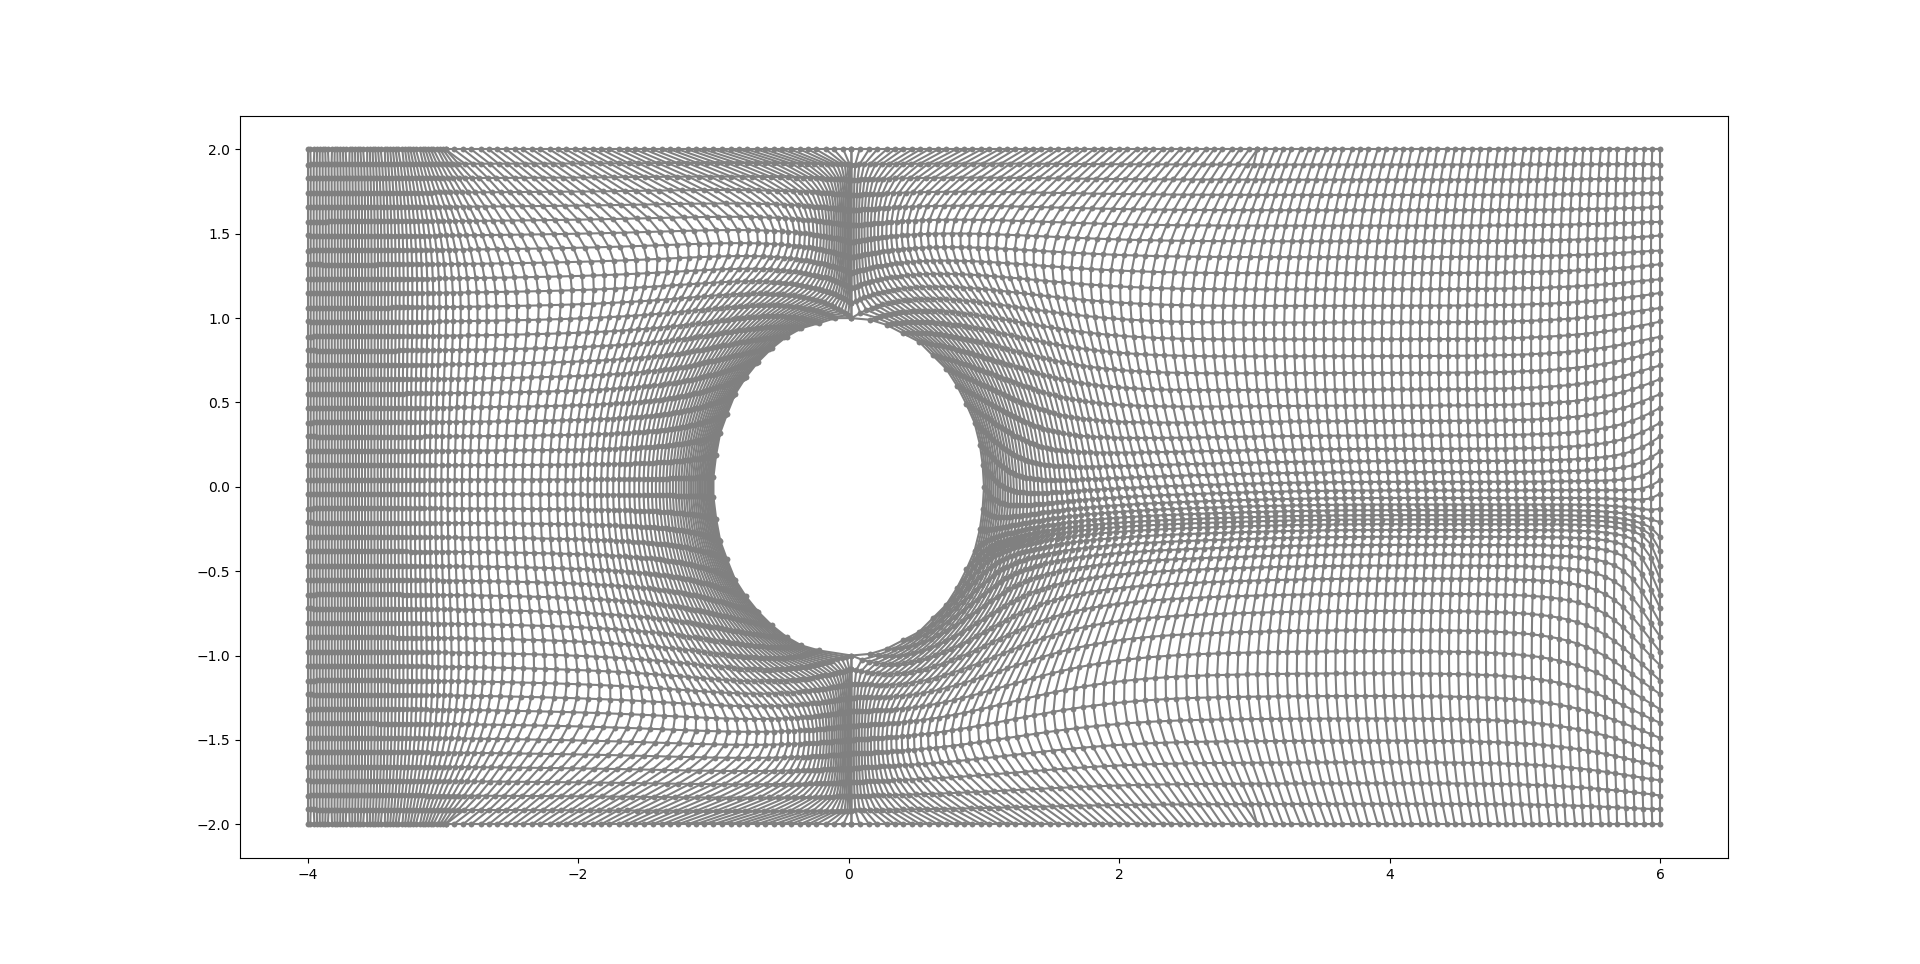
\includegraphics[width=1.0\textwidth]{heuristica_2_50pts_refined.png}
	\label{fig:heuristic2_100pts_refined} 
	\caption[caption]{Malha gerada pela heurística 2 com 50 pontos com refinamento.}
\end{figure}


%
%\subsection{Aerofólio}
%
%Código para gerar uma malha para a curva \textit{naca012}, a resolução da malha é determinada pela quantidade de pontos na curva. O domínio com comprimento 4, altura 6, e comprimento 1 à direita da curva. O domínio é divido em 4 partes, e o refinamento é feito ao redor da curva e após a curva no centro do domínio em relação à \textit{y}, ou $\eta$.
%
%
%Código utilizando a heurística 1.
%\begin{verbatim}
%imp.reload(pjt);  
%grid = pjt.generate_grid(filename_curve="naca012.txt", 
%left_border=1, domain_length=4, domain_height=3,
%heuristic=pjt.heuristic_1, k=3, filename_borders="naca012_h1", 
%xis_rf0=[1], xis_rf1=[0], etas_rf1=[0.419], a_xis0=[5], 
%a_xis1=[2.5], c_xis0=[5], c_xis1=[5], a_etas1=[5], c_etas1=[15])
%\end{verbatim}
%
%Código utilizando a heurística 2.
%\begin{verbatim}
%imp.reload(pjt);  
%grid = pjt.generate_grid(filename_curve="naca012.txt", 
%left_border=1, domain_length=4, domain_height=3,
%heuristic=pjt.heuristic_2, k=3, filename_borders="naca_h2", 
%xis_rf0=[1], xis_rf1=[0], etas_rf1=[0.419], a_xis0=[5], 
%a_xis1=[2.5], c_xis0=[5], c_xis1=[5], a_etas1=[5], c_etas1=[15])
%\end{verbatim}
%
%
%\begin{figure}[H]
%	\centering
%	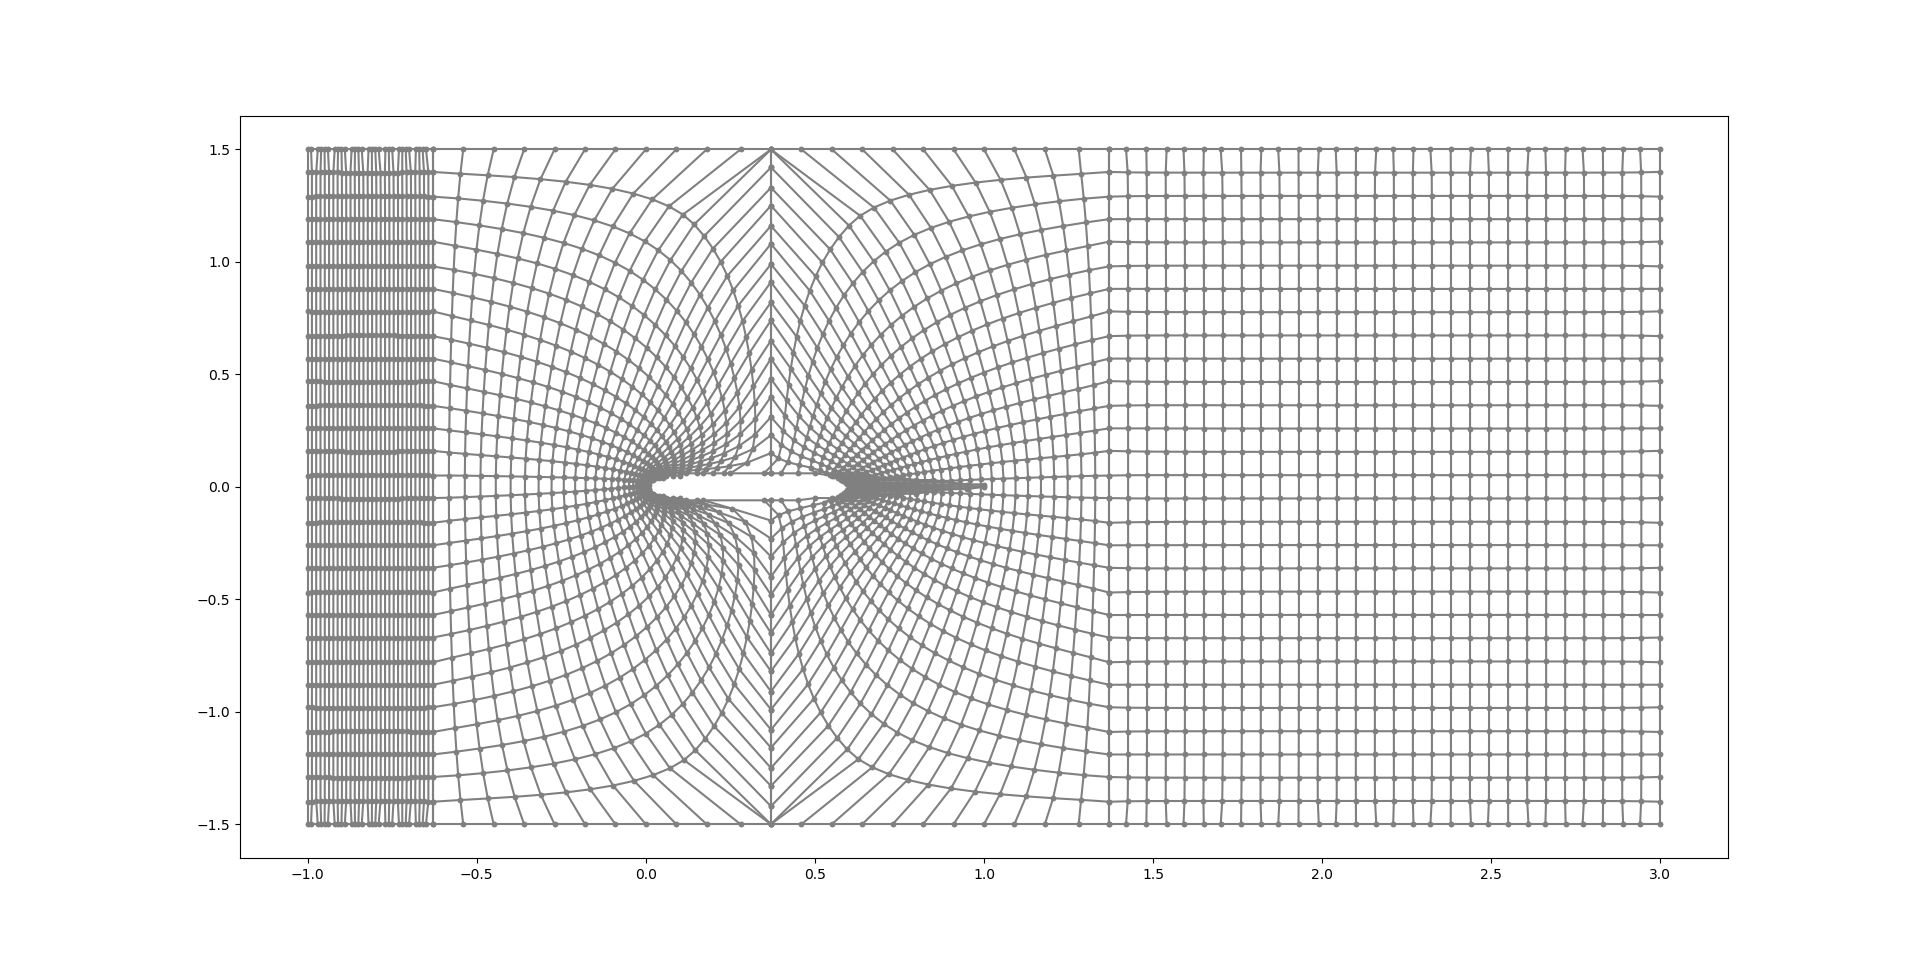
\includegraphics[width=1.0\textwidth]{naca_h1.png}
%	\label{fig:naca_h1} 
%	\caption[caption]{Malha gerada para a curva \textit{naca012 } pela heurística 1 sem refinamento.}
%\end{figure}
%
%\begin{figure}[H]
%	\centering
%	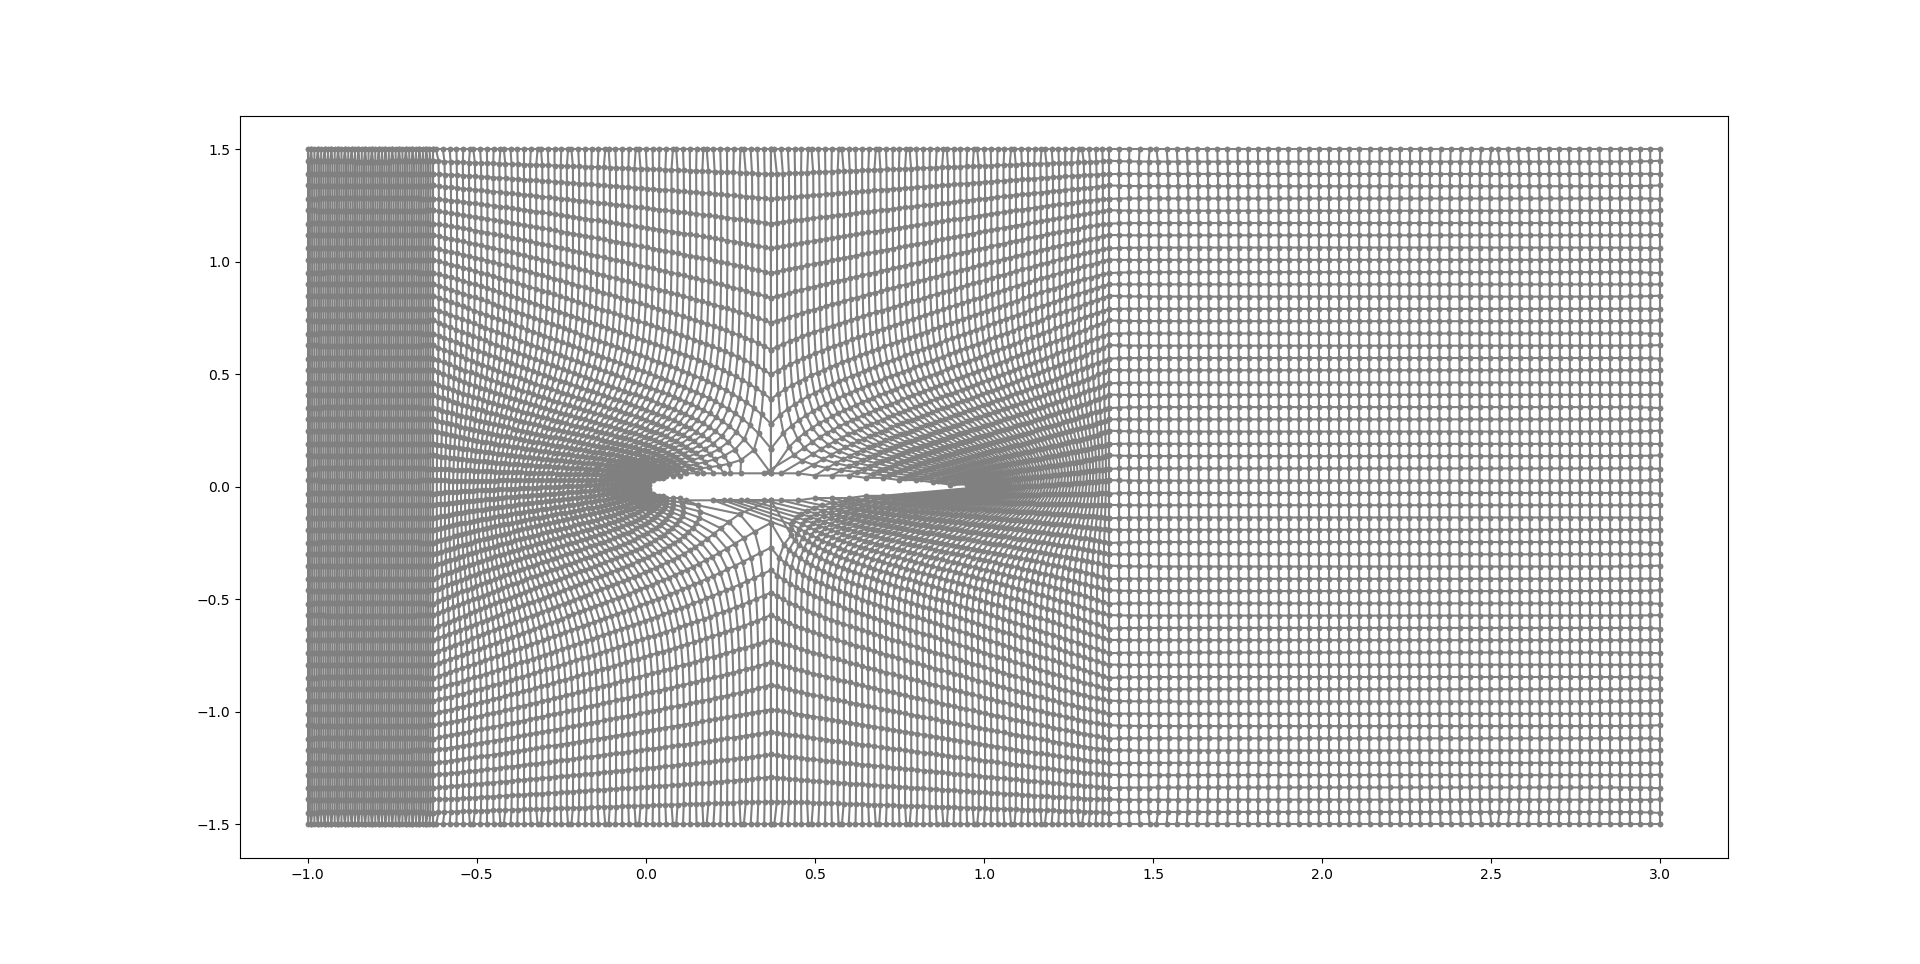
\includegraphics[width=1.0\textwidth]{naca_h2.png}
%	\label{fig:naca_h2} 
%	\caption[caption]{Malha gerada para a curva \textit{naca012 } pela heurística 2 sem refinamento.}
%\end{figure}
%
%
%
%\begin{figure}[H]
%	\centering
%	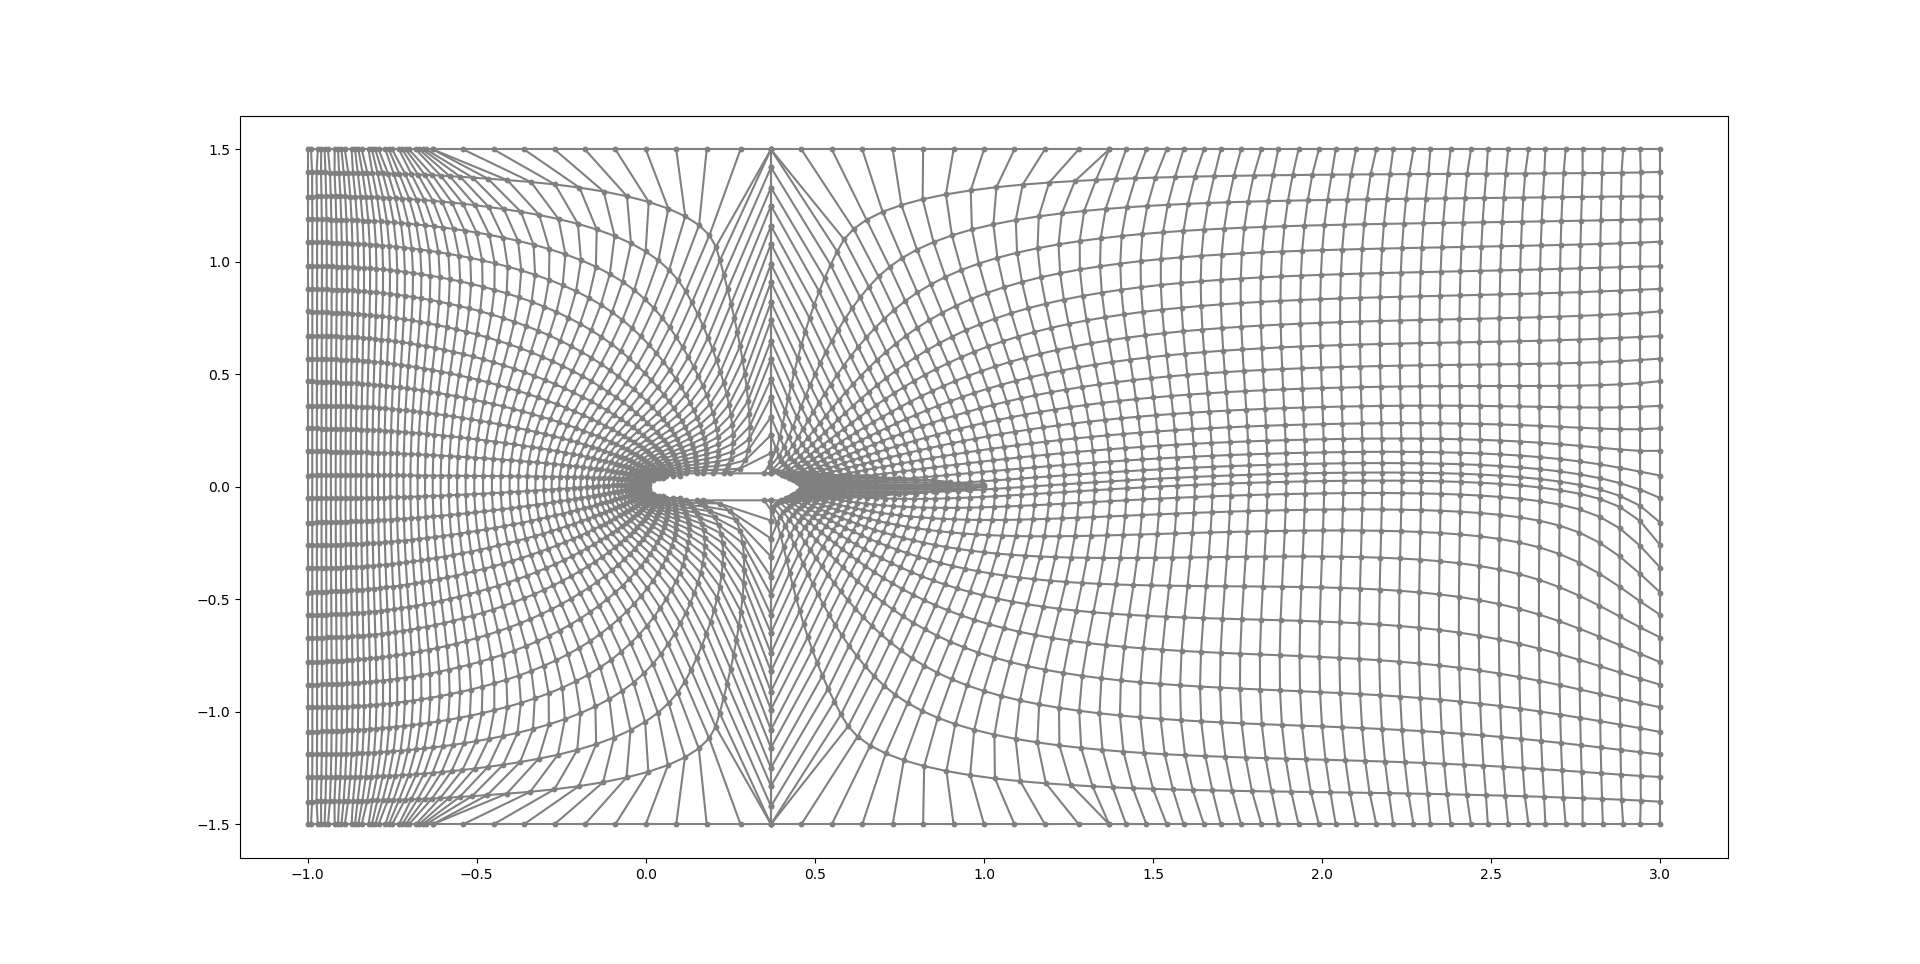
\includegraphics[width=1.0\textwidth]{naca_h1_refined.png}
%	\label{fig:naca_h1_refined} 
%	\caption[caption]{Malha gerada para a curva \textit{naca012 } pela heurística 1 com refinamento.}
%\end{figure}
%
%\begin{figure}[H]
%	\centering
%	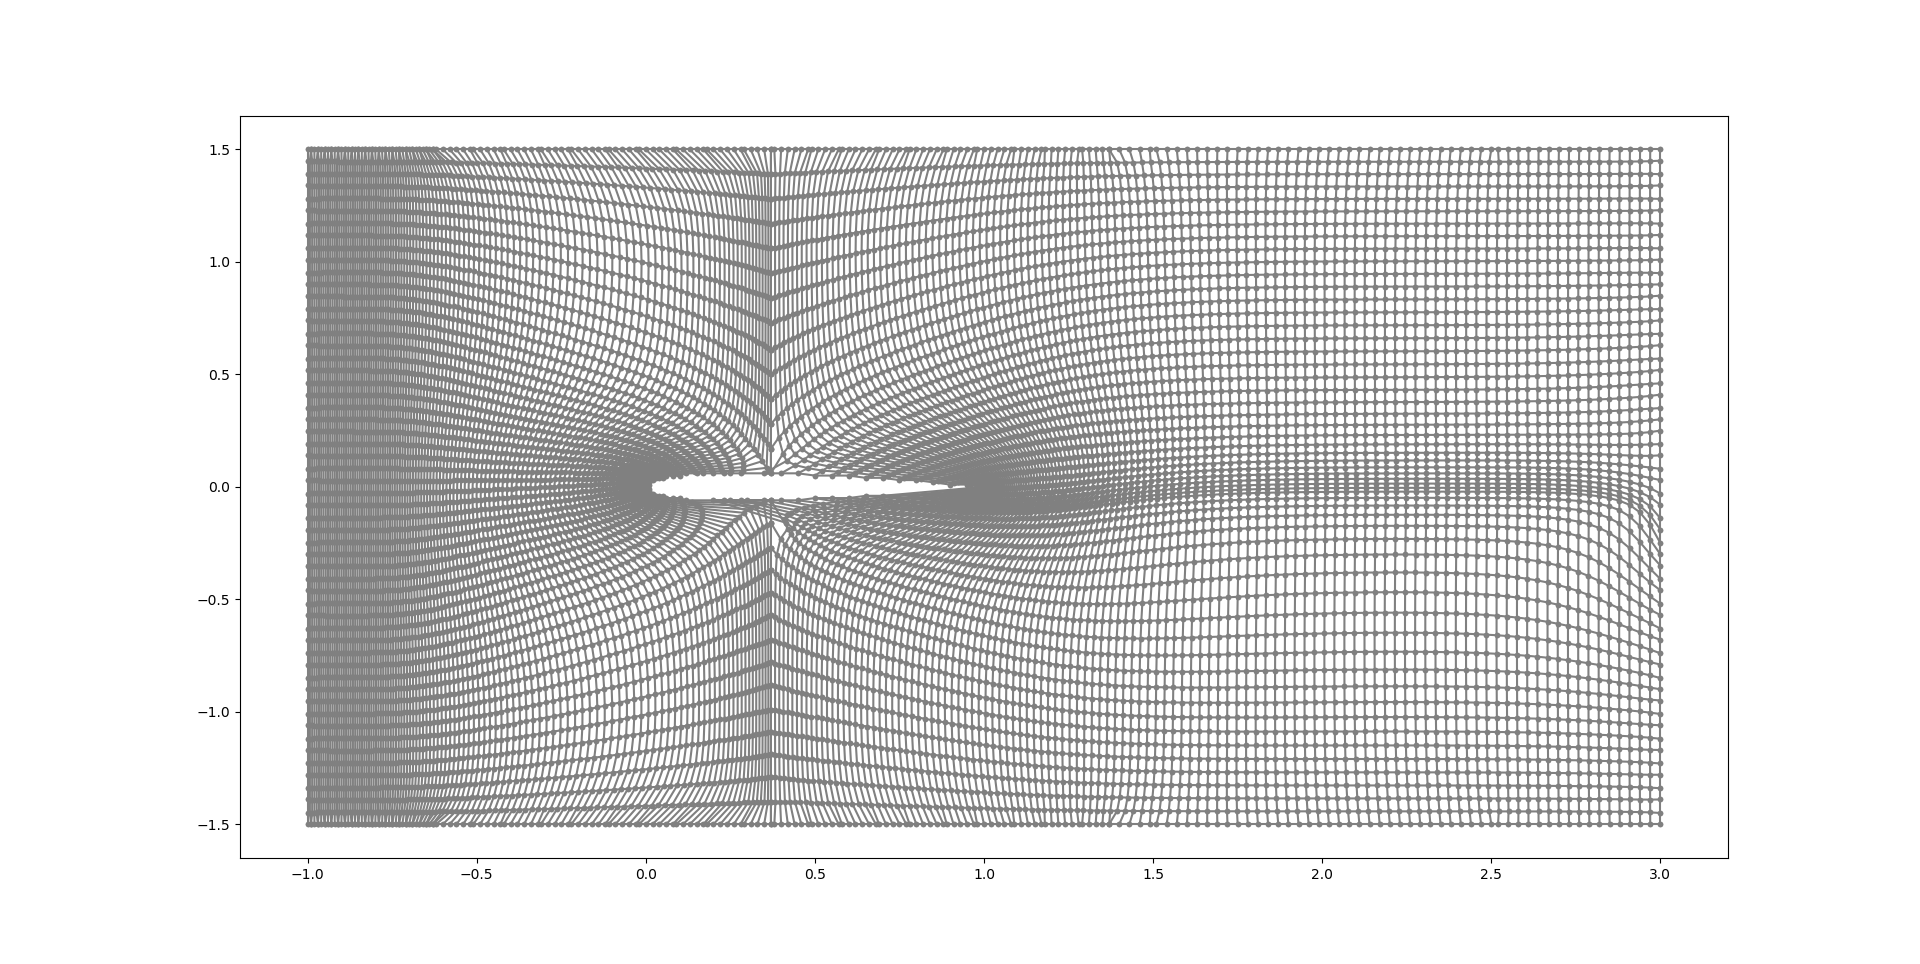
\includegraphics[width=1.0\textwidth]{naca_h2_refined.png}
%	\label{fig:naca_h2_refined} 
%	\caption[caption]{Malha gerada para a curva \textit{naca012 } pela heurística 2 com refinamento.}
%\end{figure}





\end{document}
